%%
\documentclass[a4paper,12pt,openright,twoside]{book}

\usepackage[latin1]{inputenc}
\usepackage[T1]{fontenc}
\usepackage[portuges, brazil]{babel}    % hiphena��o em portugues

%% Minah definiciones

\usepackage{xcolor} % Required for specifying colors by name
\definecolor{ocre}{RGB}{243,102,25} % Define the orange color used for highlighting throughout the book

\usepackage{color}


\definecolor{dkred}{rgb}{0.6,0,0}
\definecolor{dkgreen}{rgb}{0,0.6,0}
\definecolor{dkblue}{rgb}{0,0,0.6}
\definecolor{mygray}{rgb}{0.5,0.5,0.5}
\definecolor{mylowgray}{rgb}{0.9,0.9,0.9}
\definecolor{myverylowgray}{rgb}{0.95,0.95,0.95}
\definecolor{mymauve}{rgb}{0.58,0,0.82}
\definecolor{lavender}{rgb}{1.00,0.94,0.96}





\usepackage{natbib}  % citações tipo  [nome-ano]
\usepackage{nomencl} % glossario

\usepackage{graphicx}
\usepackage{wrapfig}
\usepackage{caption}
\usepackage{subcaption}

\usepackage{times}

\usepackage{indentfirst}  % indenta primeiro parágrafo
\usepackage{wasysym}
\usepackage{pifont}
\usepackage{textcomp}      % \texttrademark

\usepackage{url}  
\usepackage{multirow}  
\usepackage{setspace}


%Capitulos divertidos 
%Options: Sonny, Lenny, Glenn, Conny, Rejne, Bjarne, Bjornstrup
\usepackage[Lenny]{fncychap}%%Lenny funciona con htlatex algunso otros NO


%----------------------------------------------------------------------------------------
%	HYPERLINKS IN THE DOCUMENTS
%----------------------------------------------------------------------------------------
\usepackage{hyperref}
\hypersetup{
%    colorlinks=true,
%    linkcolor=blue,
%    filecolor=magenta,      
%    urlcolor=cyan,
%    pdftitle={Sharelatex Example},
    bookmarks=true,
%    pdfpagemode=FullScreen,
}

\usepackage{fancyhdr}

%% tamanho do texto e margens
\setlength{\topmargin}{-15pt} % extra vert. space + at the top of header: 23pt
\setlength{\oddsidemargin}{0pt} % extra spc added at the left of odd page: 0pt
\setlength{\evensidemargin}{-12pt} % ext. spc added at the left of even pg: 59pt
\setlength{\textheight}{638pt} % height of the body: 592pt
\setlength{\textwidth}{483pt} % width of the body: 470pt

%% Estilo da página corrente e demais páginas
\pagestyle{fancyplain}
\renewcommand{\chaptermark}[1]{\markboth{#1}{}}
\renewcommand{\sectionmark}[1]{\markright{\thesection\ #1}}
\lhead[\fancyplain{}{\bfseries\thepage}]{\fancyplain{}{\bfseries\rightmark}}
\rhead[\fancyplain{}{\bfseries\leftmark}]{\fancyplain{}{\bfseries\thepage}}
\cfoot[\fancyplain{\bfseries\thepage}{}]{\fancyplain{\bfseries\thepage}{}}

\usepackage{listings}
\lstset{
  language=C,%linguagem por defeito
  frame=tb,
  classoffset=0,
  %otherkeywords={..,;,=,<,>,<=,=>,==},%%%NO HABILITAR SI UAS HTLATEX
  keywordstyle=\color{dkred},
  classoffset=0,
  %
  commentstyle=\color{dkgreen},
  %
  stringstyle=\color{mymauve},
  captionpos=b,
  %
  aboveskip=3mm,
  belowskip=3mm,
  backgroundcolor=\color{myverylowgray},
  showstringspaces=false,
  columns=flexible,
  basicstyle={\small\ttfamily},
  %
  numbers=none,
  numberstyle=\tiny\color{mygray},
  %
  breaklines=true,
  breakatwhitespace=true,
  tabsize=4
}


%% Para a cria��o do Gloss�rio
\makenomenclature

\newtheorem{theorem}{Theorema}
\newtheorem{definition}{Defini��o}
\newtheorem{informationbox}{Informa��o}

\usepackage{tasks}

%%%%%%%%%%%%%%%%%%%%%%%%%%%%%%%%%%%%%%%%%%%%%%%%%%%%%%%%%%%%%%%%%%%%%%%%%%%%%%%%
%% Inicia o texto
\begin{document}


%% Paginas iniciais (sem numera��o)
\frontmatter

%% P�gina de rosto

\begin{comment}
\begin{titlepage}
\maketitle
\end{titlepage} 
\end{comment}

%% \begin{comment}
\begin{titlepage}
\begin{center}
%% Upper part of the page
%\includegraphics[width=1\textwidth]{./up-logo.jpg}\\[0.4cm]    
\textsc{\LARGE Primeira Edição}\\[1.0cm]

\includegraphics[width=0.3\textwidth]{principal}\\[1.0cm]
%% pretitle
%{\fontsize{25}{30} \textsc{Algum pretitulo}}
%% Title
\HRule{0.4cm} \\[0.4cm]
{ \fontsize{50}{60}   \bfseries \mytitle}\\[0.4cm]
\HRule{0.4cm} \\[0.7cm]
%% SubTitle
{\fontsize{25}{30} \textsc{\mysubtitle}}\\[0.5cm]
\vfill
%% Author 
\begin{minipage}{0.4\textwidth}
\begin{flushleft} \large
%\emph{Author:}\\
\myauthor %\textsc{Coppejans}
\end{flushleft}
\end{minipage}
% ID
\begin{minipage}{0.4\textwidth}
\begin{flushright} \large
\emph{email:} \\
\ImprimirEmail
\end{flushright}
\end{minipage}
% Bottom of the page
\vfill
{\large \imprimirdata}
\end{center}
\end{titlepage}
%% \end{comment}

%% Lista de conte�do (sum�rio)
\def\contentsname{Sumario}
\tableofcontents

%% Lista de figuras (gerada automaticamente)
\cleardoublepage
\addcontentsline{toc}{chapter}{Lista de Figuras}
\listoffigures

%% Lista de tabelas (gerada automaticamente)
%\cleardoublepage
\addcontentsline{toc}{chapter}{Lista de Tablas}
\listoftables

%% Gloss�rio (gerado automaticamente - veja entradas em cap1.tex)
\cleardoublepage

\renewcommand{\nomname}{Glosario}
\markboth{GLOSARIO}{GLOSARIO}


\addcontentsline{toc}{chapter}{\nomname}
\printnomenclature

%% Lista de Simbolos (gerada manualmente)
%\cleardoublepage
\addcontentsline{toc}{chapter}{Lista de S�mbolos}

\markboth{LISTA DE S�MBOLOS}{LISTA DE S�MBOLOS}

\chapter*{Lista de S�mbolos}

\singlespacing

\noindent
\begin{tabular}{l c p{.85\linewidth}}
$M$ & - & N�mero de ramos de diversidade \\
$r_i$ & - & Envolt�ria do $i$-�simo ramo \\
$\hat{r}_i$ & - & Valor rms de $r_i$ \\
$\rho_i$ & - & Envolt�ria do $i$-�simo ramo, normalizada em rela��o a $\hat{r}_i$ \\
$p(x)$ & - & Fun��o densidade de probabilidade da vari�vel aleat�ria $x$ \\
$P(x)$ & - & Fun��o distribui��o de probabilidade da vari�vel aleat�ria $x$ \\
$m_i$ & - & Par�metro de Nakagami-\emph{m} do $i$-�simo ramo \\
$\mathrm{E} (\cdot)$ & - & M�dia de uma vari�vel aleat�ria \\
$\mathrm{Var} (\cdot)$ & - & Vari�ncia de uma vari�vel aleat�ria \\
$k_i$ & - & Par�metro de Rice do $i$-�simo ramo \\
$\dot{r}_i$ & - & Derivada temporal de $r_i$ \\
$\dot{\rho}_i$ & - & Derivada temporal de $\rho_i$ \\
$p(x,y)$ & - & Fun��o densidade de probabilidade conjunta das vari�veis aleat�rias $x$ e $y$ \\
\end{tabular}

\onehalfspacing


\mainmatter

%% Cap. 1 - Introdu��o
%%
%% Cap�tulo 1: Modelo de Cap�tulo
%%
\chapter{Modelo de cap�tulo}
\label{Cap:modelo}

%%%%%%%%%%%%%%%%%%%%%%%%%%%%%%%%%%%%%%%%%%%%%%%%%%%%%%%%%%%%%%%%%%%%%%%%%%%%%%%%
%%%%%%%%%%%%%%%%%%%%%%%%%%%%%%%%%%%%%%%%%%%%%%%%%%%%%%%%%%%%%%%%%%%%%%%%%%%%%%%%
\section{Posi��es}
\label{Sec:posicoes} 
\begin{tasks}(2)
\task \textbf{Posi��o frente a frente direita (FFD):} 
\task \textbf{Posi��o frente a frente esquerda (FFE):}
\task \textbf{Posi��o frente a frente frente (FFF):} 
\task \textbf{Posi��o frente a frente atras (FFA):}
\task \textbf{Posi��o fechada atr�s direita (FAD):}
\task \textbf{Posi��o fechada atr�s esquerda (FAE):}
\task \textbf{Posi��o de X (X):}  
\task \textbf{Posi��o de X complemento (XC):} 
\task \textbf{Posi��o de X invertida (XI):} Figuras \ref{fig:position:xinvertido}
similar � posi��o XC, por�m com o peso do condutor e seguidor na perna direita e esquerda, respetivamente.
\task \textbf{Posi��o de fac�o (F):}
\task \textbf{Posi��o de rom�rio (R):} Figuras \ref{fig:position:r}
\task \textbf{Posi��o de esse direita (sd):} Figuras \ref{fig:position:sd}
\task \textbf{Posi��o de esse esquerda (se):} Figuras \ref{fig:position:se}
\end{tasks}

Todos as posi��es s�o vistas na Figura \ref{fig:position:all}.

\begin{figure}[!h]
     \centering
     \begin{subfigure}[b]{0.24\textwidth}
         \centering
         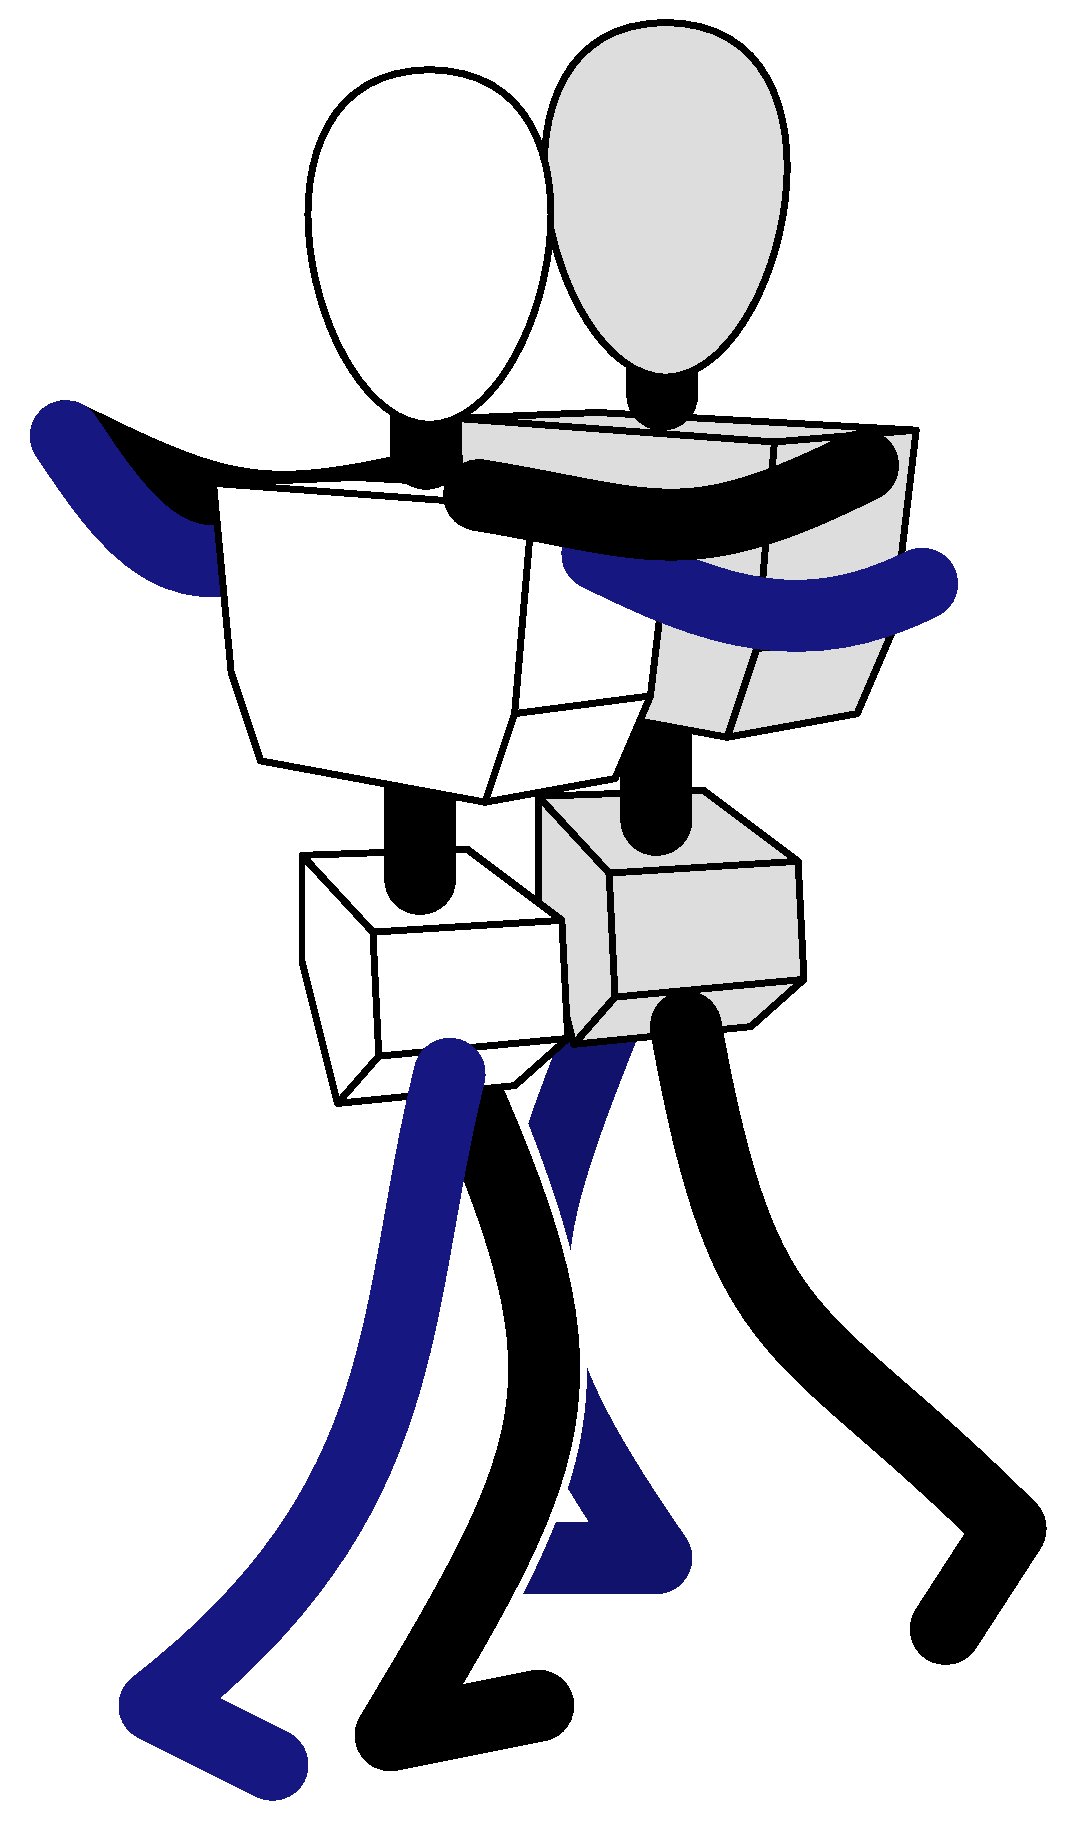
\includegraphics[width=0.9\textwidth]{caps/cap1/position-r.eps}
         \caption{Position R.}
         \label{fig:position:r}
     \end{subfigure}
     \hfill
     \begin{subfigure}[b]{0.24\textwidth}
         \centering
         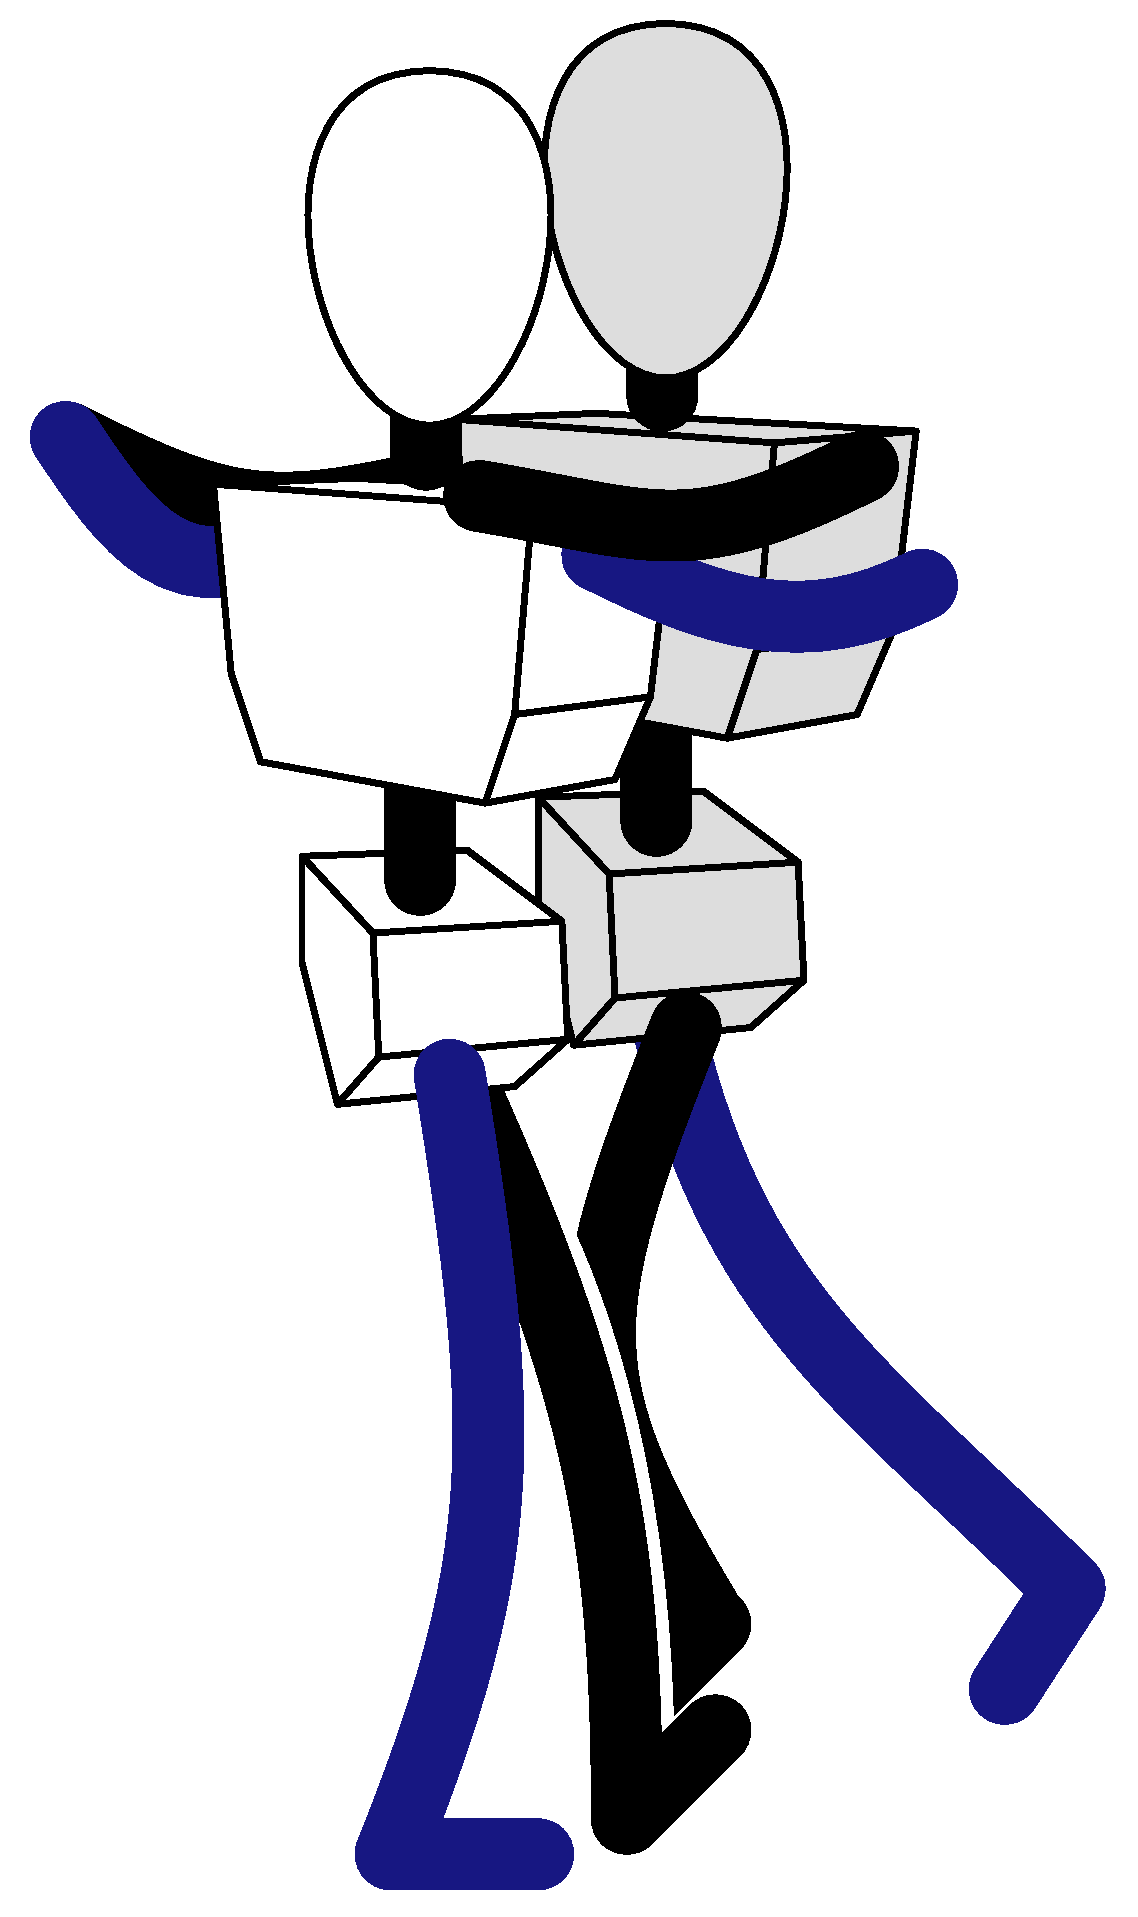
\includegraphics[width=0.9\textwidth]{caps/cap1/position-x-invertido.eps}
         \caption{Position X invertido.}
         \label{fig:position:xinvertido}
     \end{subfigure}
     \hfill
     \begin{subfigure}[b]{0.24\textwidth}
         \centering
         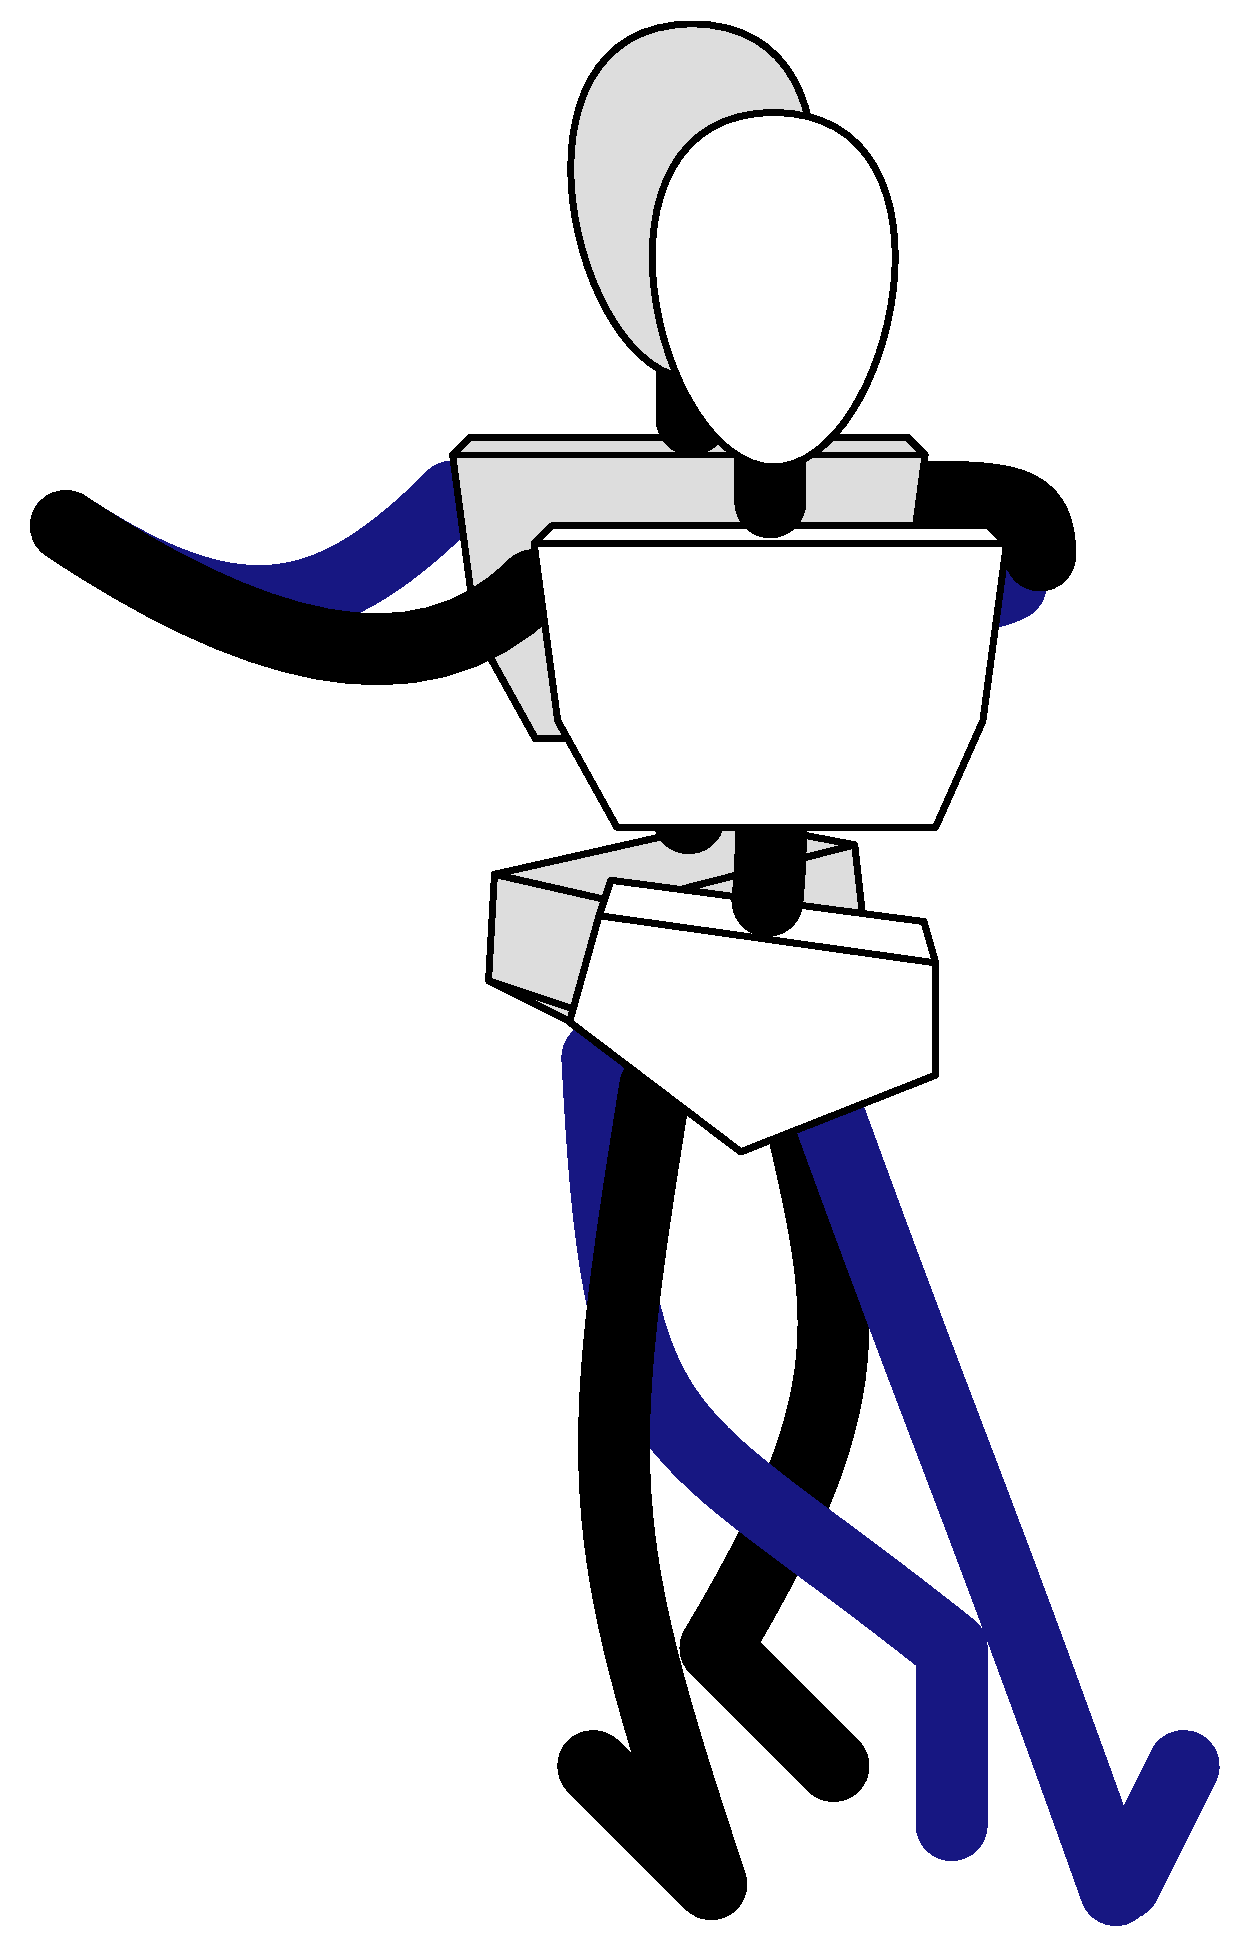
\includegraphics[width=0.9\textwidth]{caps/cap1/position-se.eps}
         \caption{Position de esse esquerda.}
         \label{fig:position:se}
     \end{subfigure}
     \hfill
     \begin{subfigure}[b]{0.21\textwidth}
         \centering
         
\includegraphics[width=0.9\textwidth]{caps/cap1/position-sd.eps}
         \caption{Position de esse direita.}
         \label{fig:position:sd}
     \end{subfigure}
        \caption{Three simple graphs}
        \label{fig:three graphs}
\end{figure}

\begin{figure}[!h]
\centering 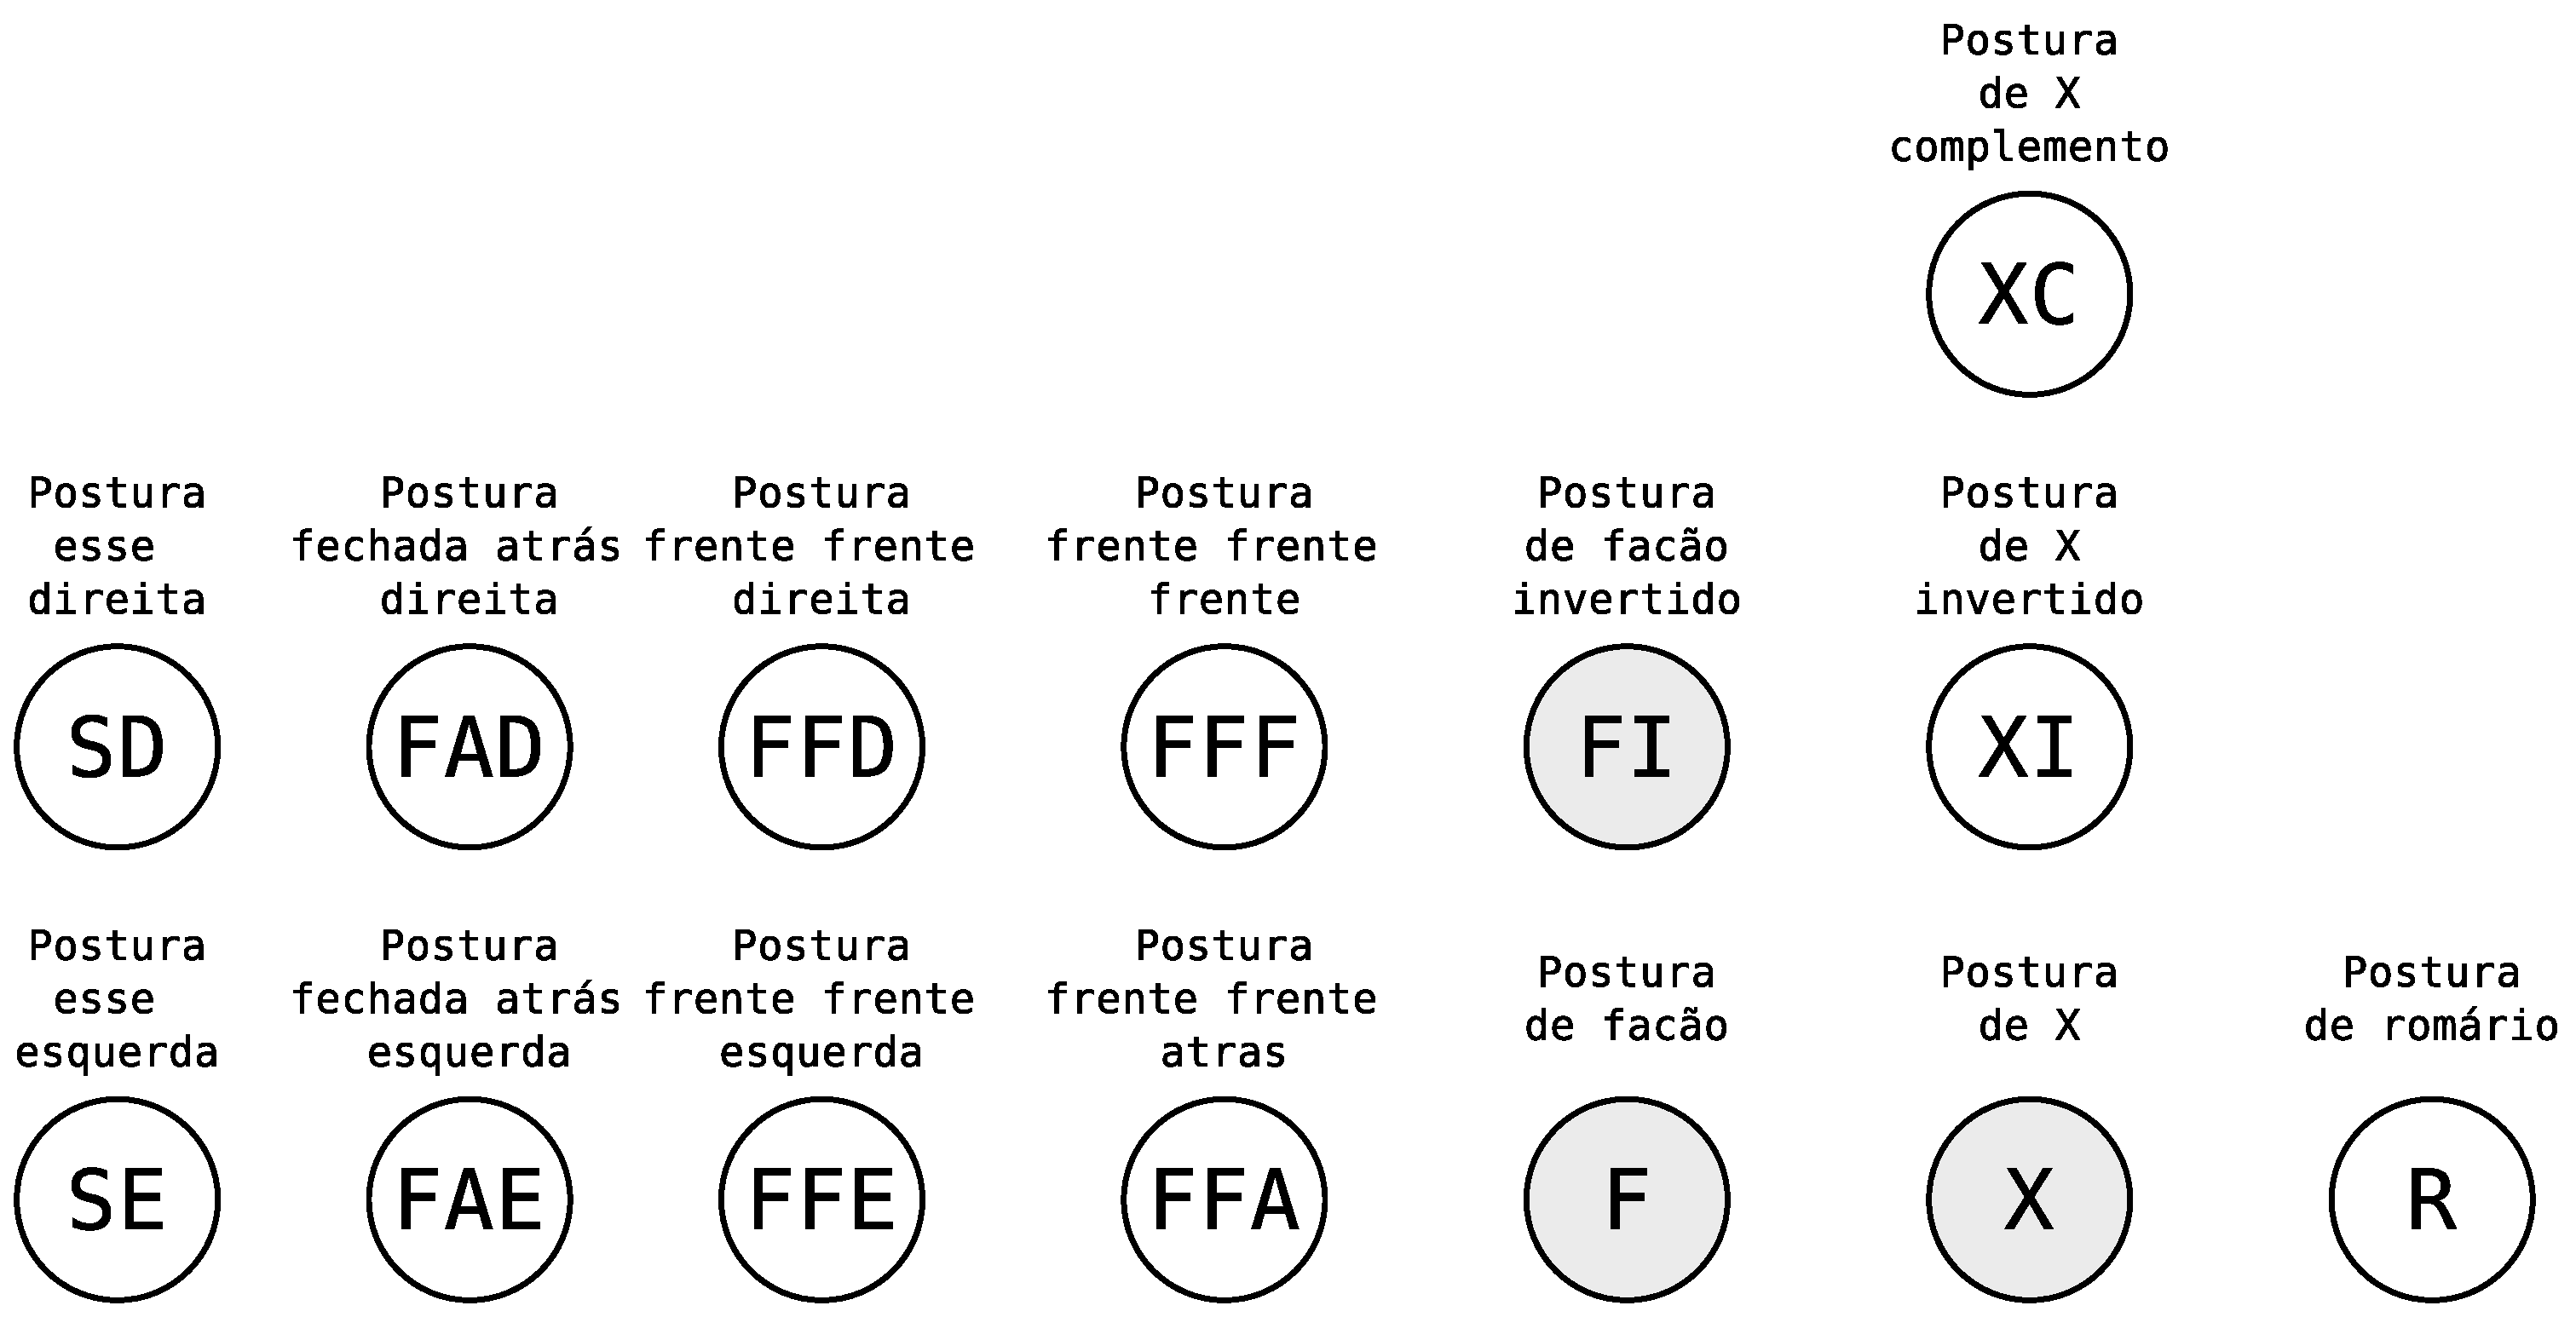
\includegraphics[width=0.99\textwidth]{caps/cap1/positions.eps}
\caption{Posi��es usadas no syllabus.}
\label{fig:position:all}
\end{figure}


%%%%%%%%%%%%%%%%%%%%%%%%%%%%%%%%%%%%%%%%%%%%%%%%%%%%%%%%%%%%%%%%%%%%%%%%%%%%%%%%
%%%%%%%%%%%%%%%%%%%%%%%%%%%%%%%%%%%%%%%%%%%%%%%%%%%%%%%%%%%%%%%%%%%%%%%%%%%%%%%%
\cleardoublepage
\section{Passos}
\label{Sec:passos} 


\subsection{Passos iniciantes}
\label{sec:passos:iniciantes}

Os passos b�sico no syllabus e as conex�es entre eles s�o vistos na Figura \ref{fig:syllabus:basico}.

\begin{figure}[!h]
\centering 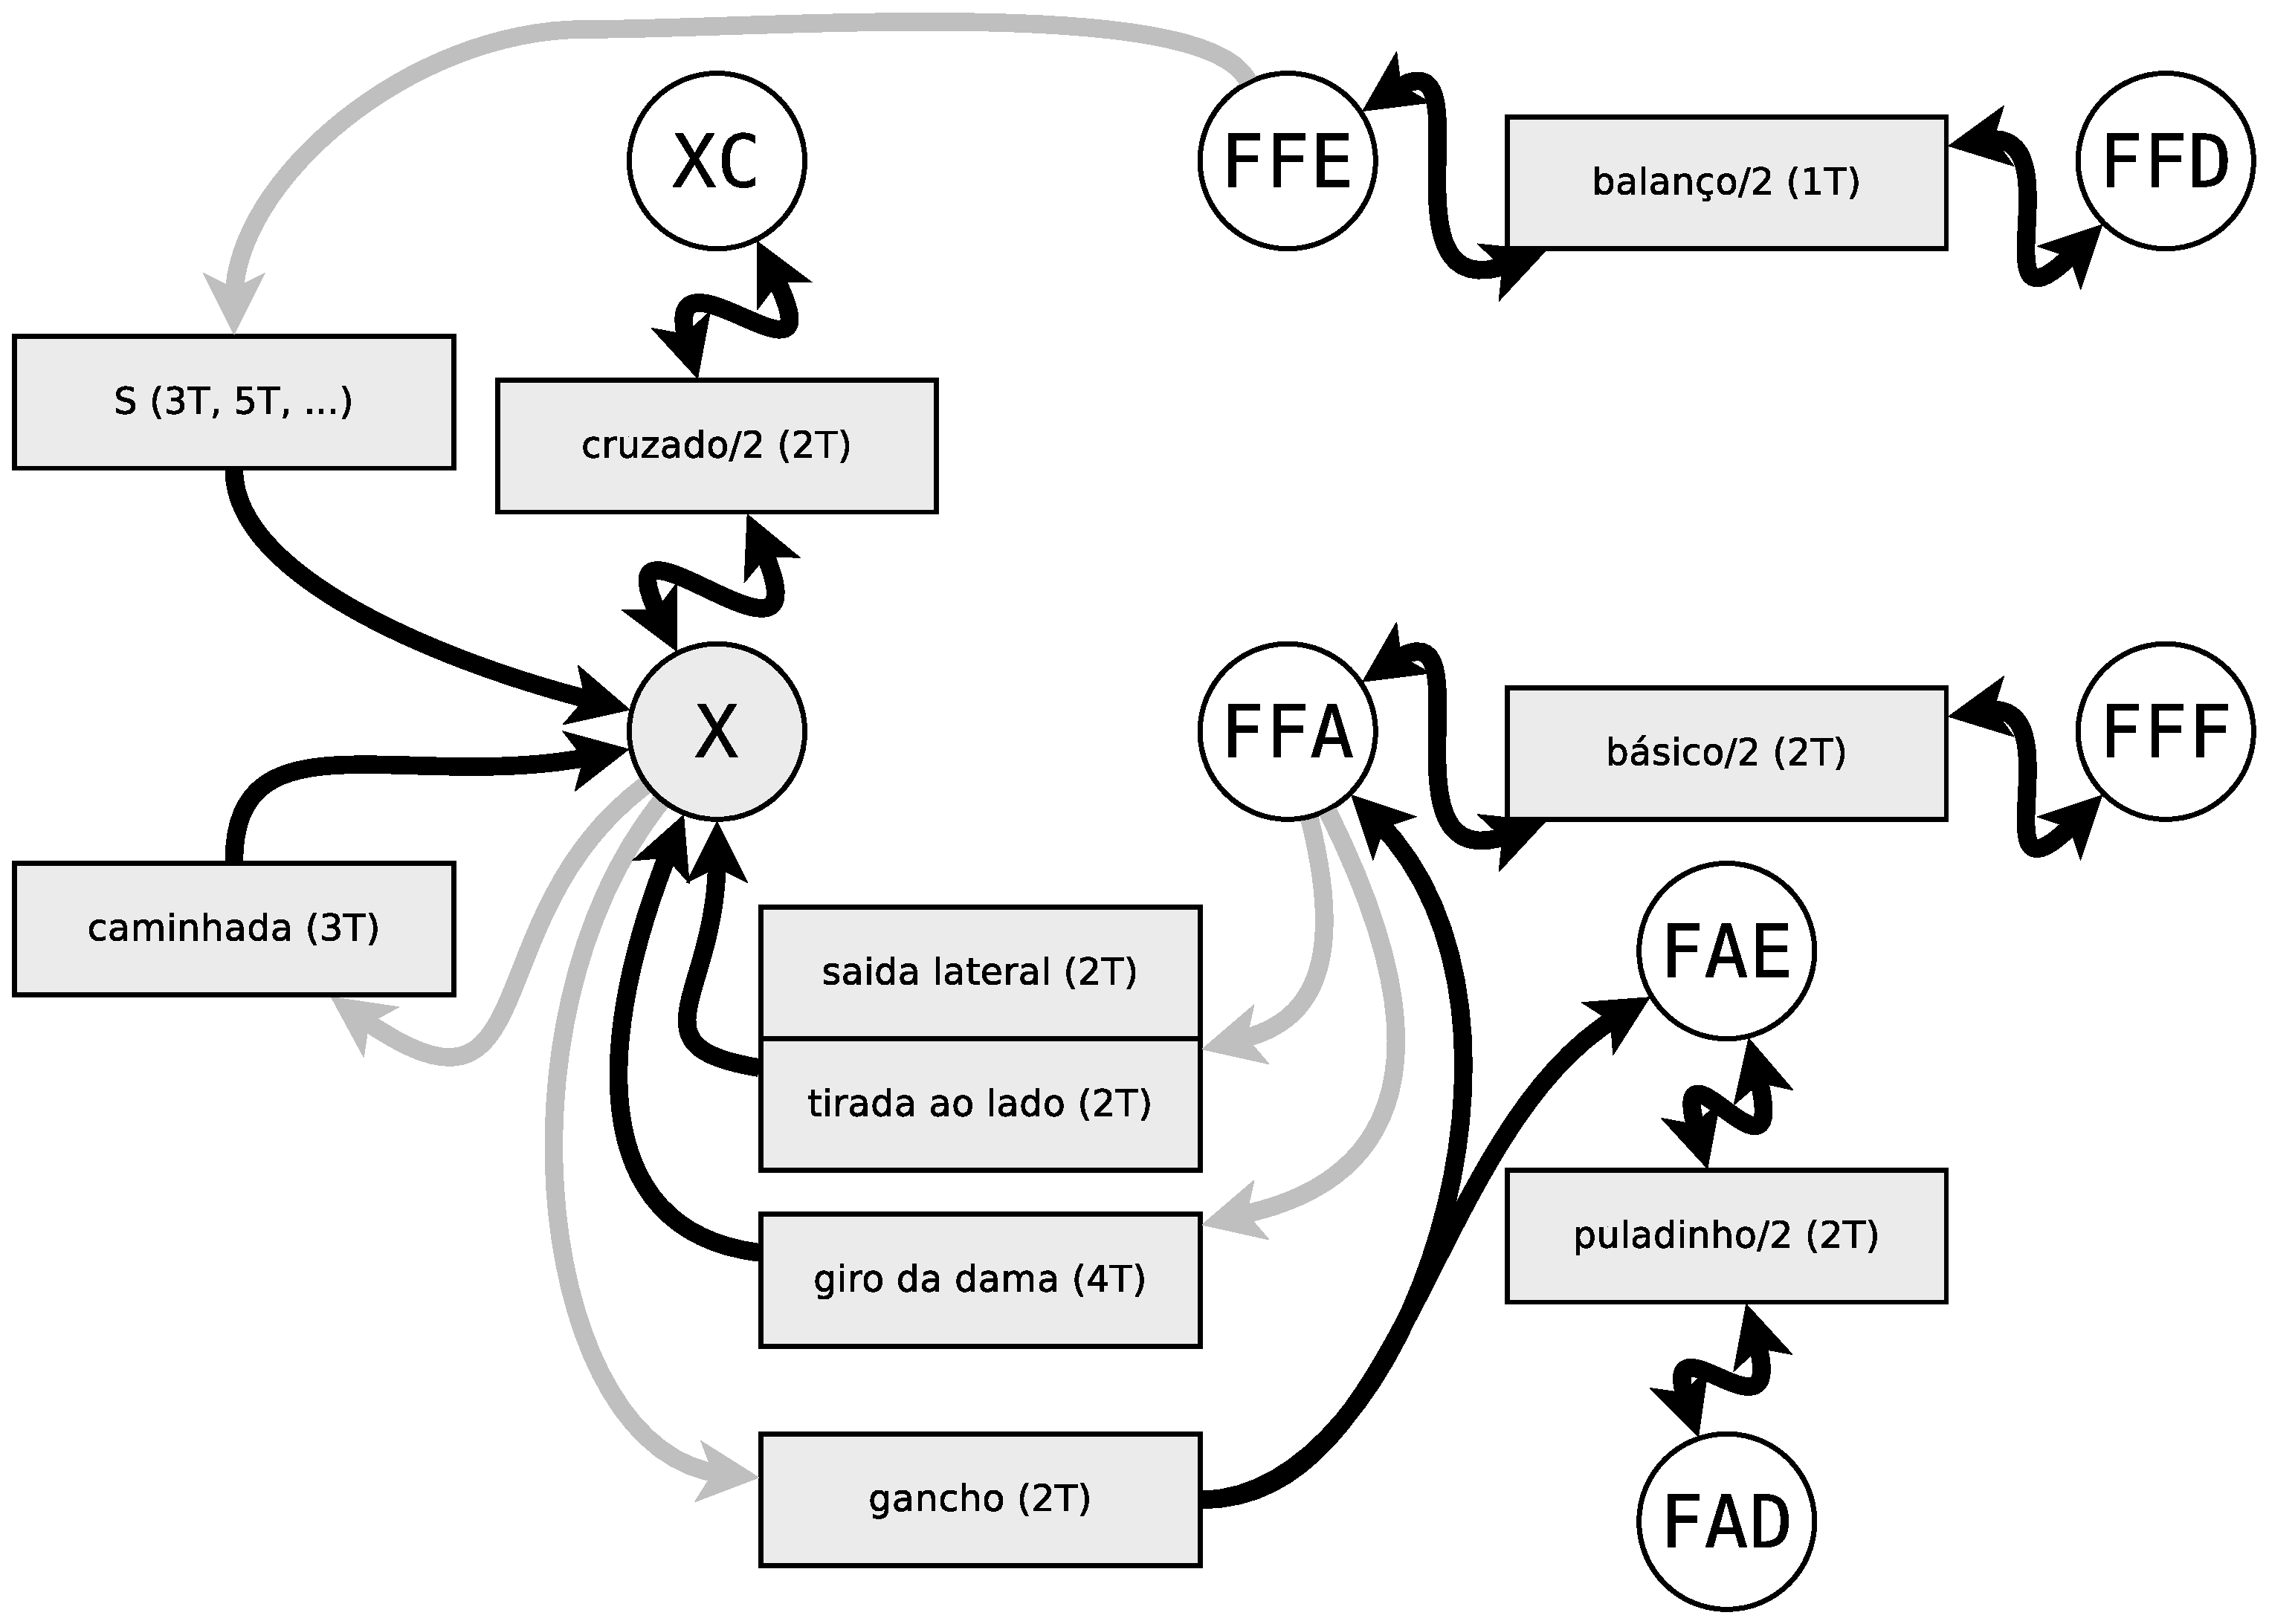
\includegraphics[width=0.8\textwidth]{caps/cap1/syllabus-basico.eps}
\caption{Passos b�sicos no syllabus.}
\label{fig:syllabus:basico}
\end{figure}

\begin{tasks}(2)
\task \textbf{B�sico:} Figura \ref{fig:passo:basico}
\task \textbf{Cruzado:} Figura \ref{fig:passo:cruzado}
\task \textbf{Gancho:} Figura \ref{fig:passo:gancho}
\task \textbf{Tirada ao lado:} Figura \ref{fig:passo:tirada-ao-lado}
\task \textbf{Saida lateral:} Figura \ref{fig:passo:saida-lateral}
\task \textbf{Balan�o:} Figura \ref{fig:passo:balanco}
\task \textbf{Caminhada:} Figura \ref{fig:passo:caminhada}
\task \textbf{Giro da dama (gatilho):} Figura \ref{fig:passo:giro-da-dama}
\task \textbf{Puladinho:} Figura \ref{fig:passo:puladinho}
\task \textbf{Esse:} da dama para tr�s desde balan�o, Figura \ref{fig:passo:esse}
\end{tasks}




\begin{figure}[!h]
\centering 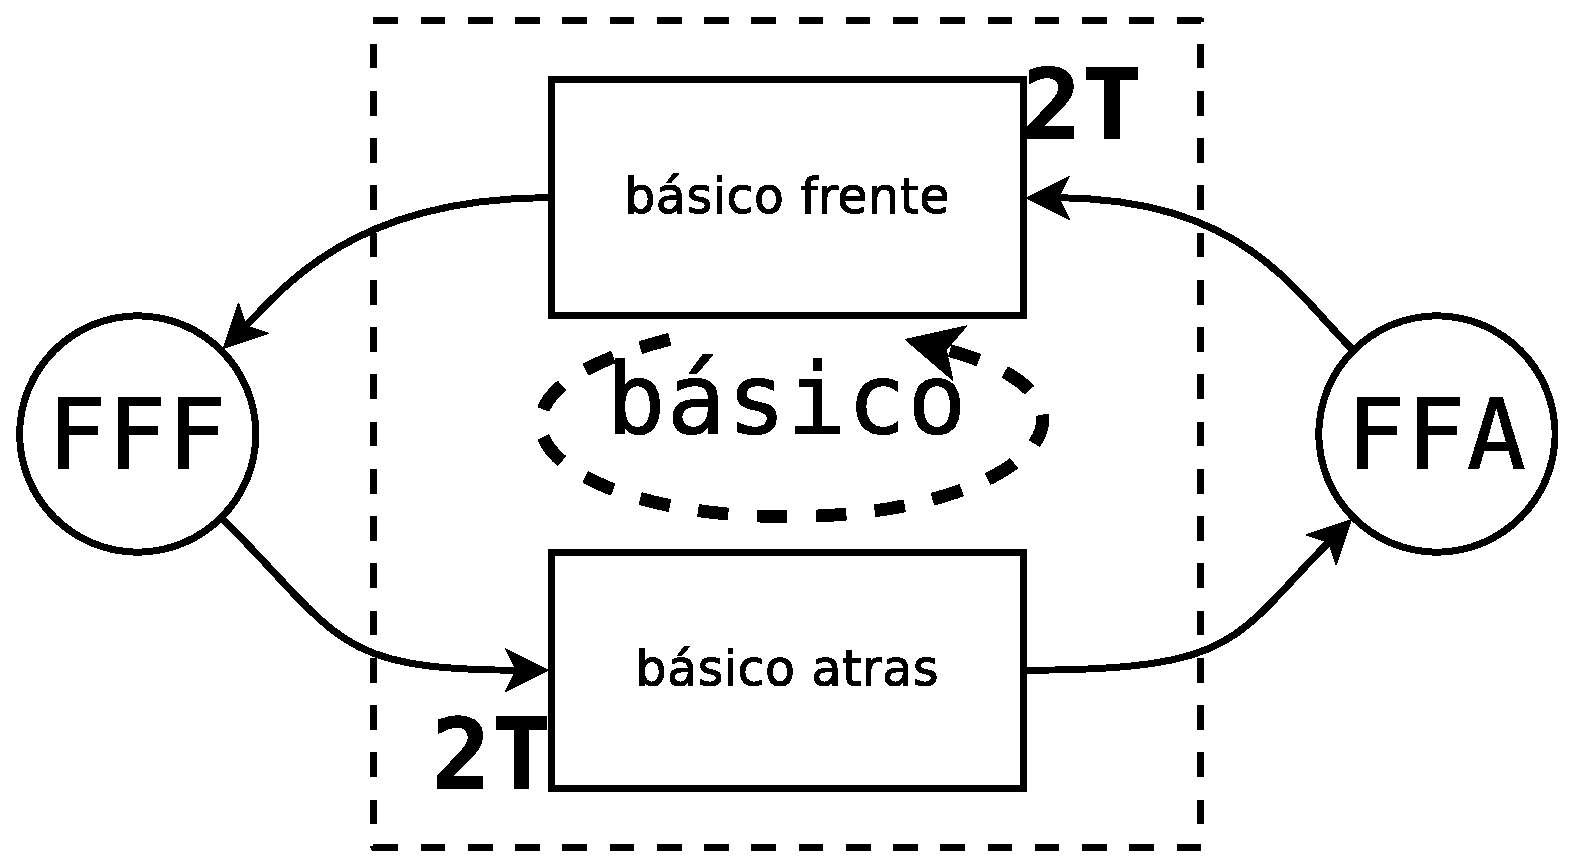
\includegraphics[width=0.5\textwidth]{caps/cap1/basico.eps}
\caption{B�sico (4T).}
\label{fig:passo:basico}
\end{figure}

\begin{figure}[!h]
\centering 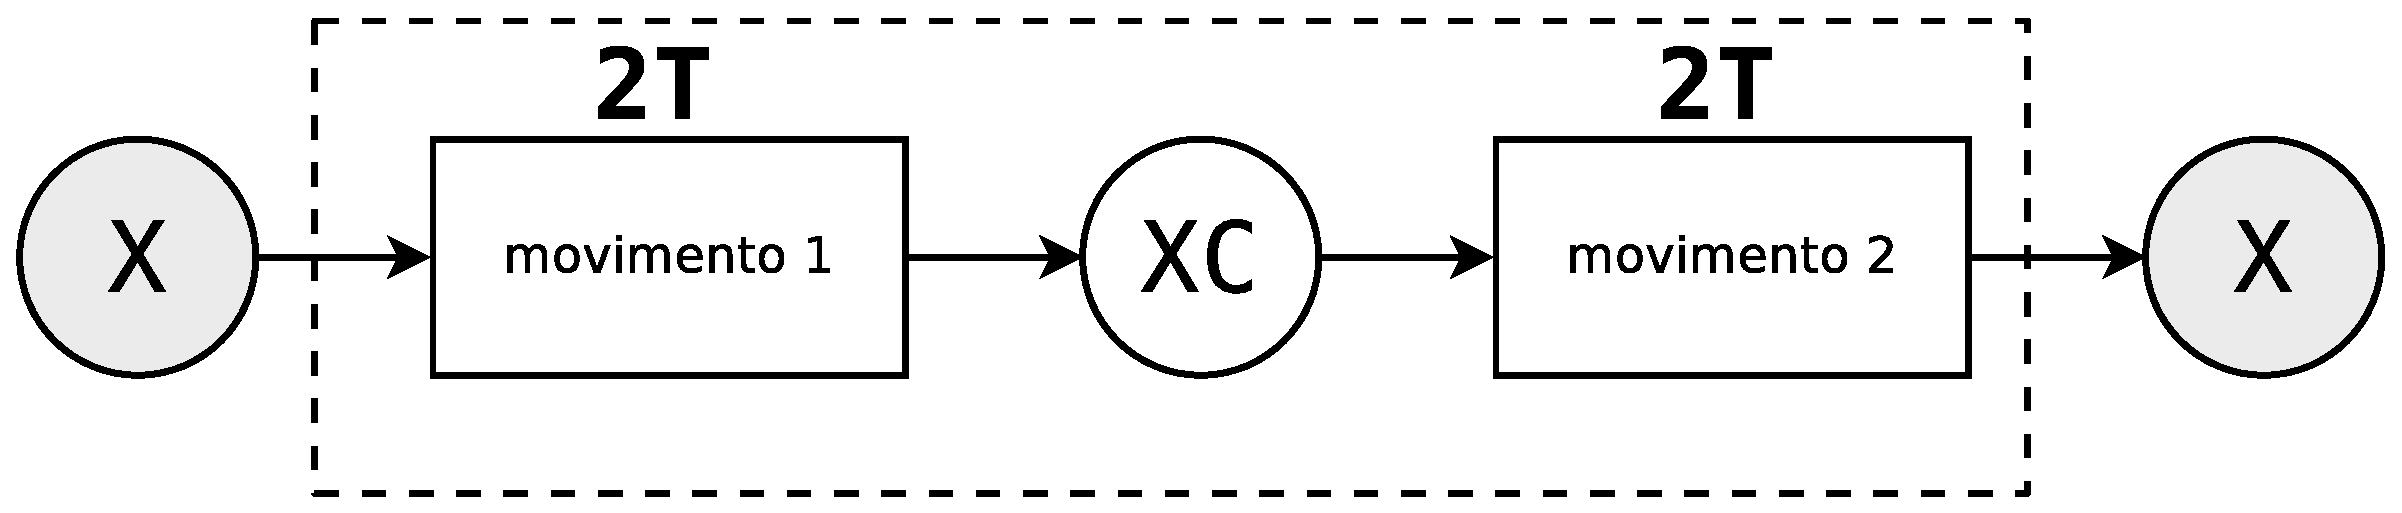
\includegraphics[width=0.75\textwidth]{caps/cap1/cruzado.eps}
\caption{Cruzado (4T).}
\label{fig:passo:cruzado}
\end{figure}

\begin{figure}[!h]
\centering 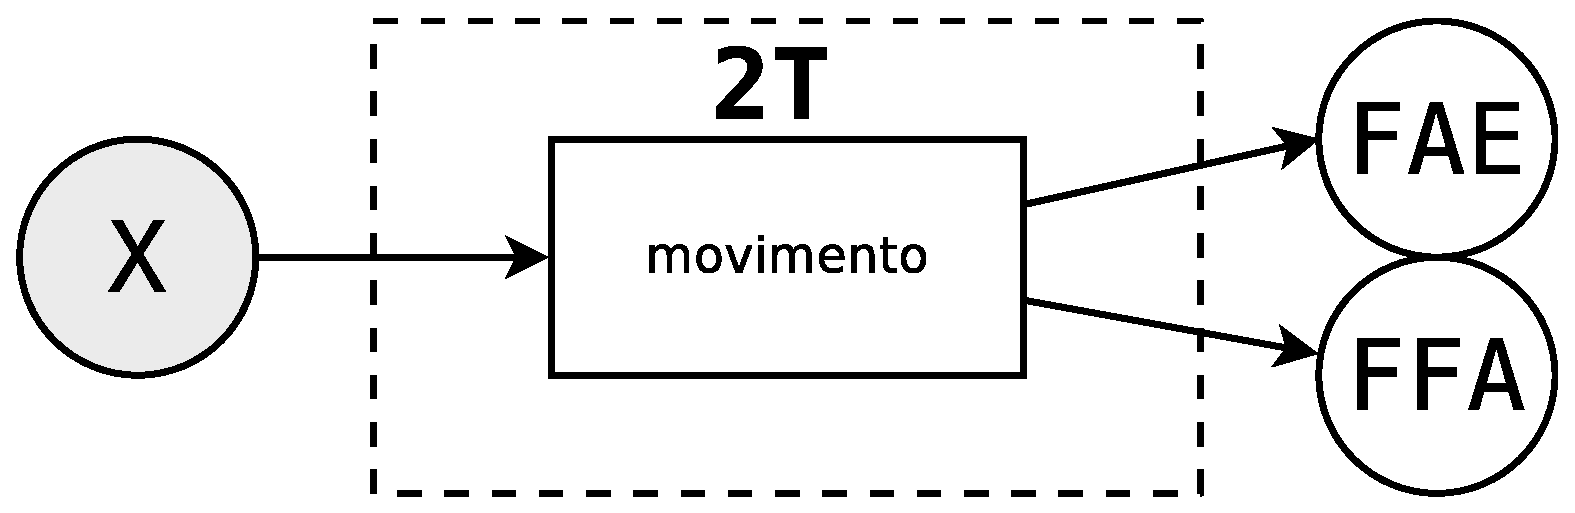
\includegraphics[width=0.5\textwidth]{caps/cap1/gancho.eps}
\caption{Gancho (2T).}
\label{fig:passo:gancho}
\end{figure}

\begin{figure}[!h]
\centering 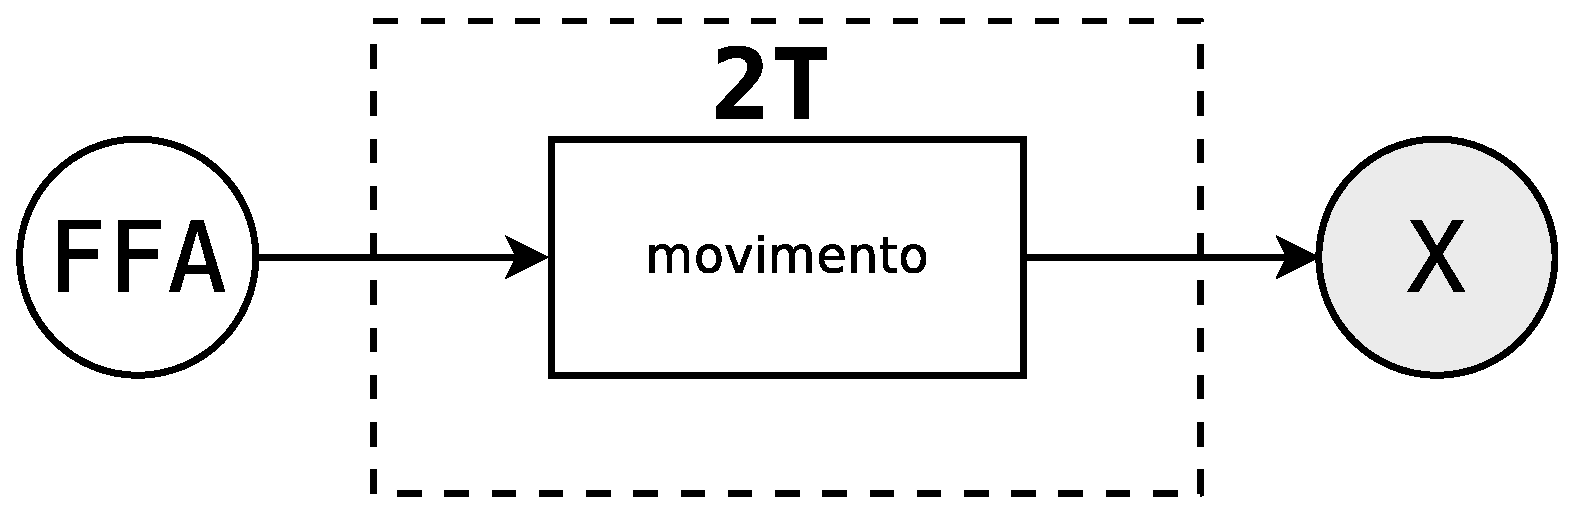
\includegraphics[width=0.5\textwidth]{caps/cap1/tirada-ao-lado.eps}
\caption{Tirada ao lado (2T).}
\label{fig:passo:tirada-ao-lado}
\end{figure}

\begin{figure}[!h]
\centering 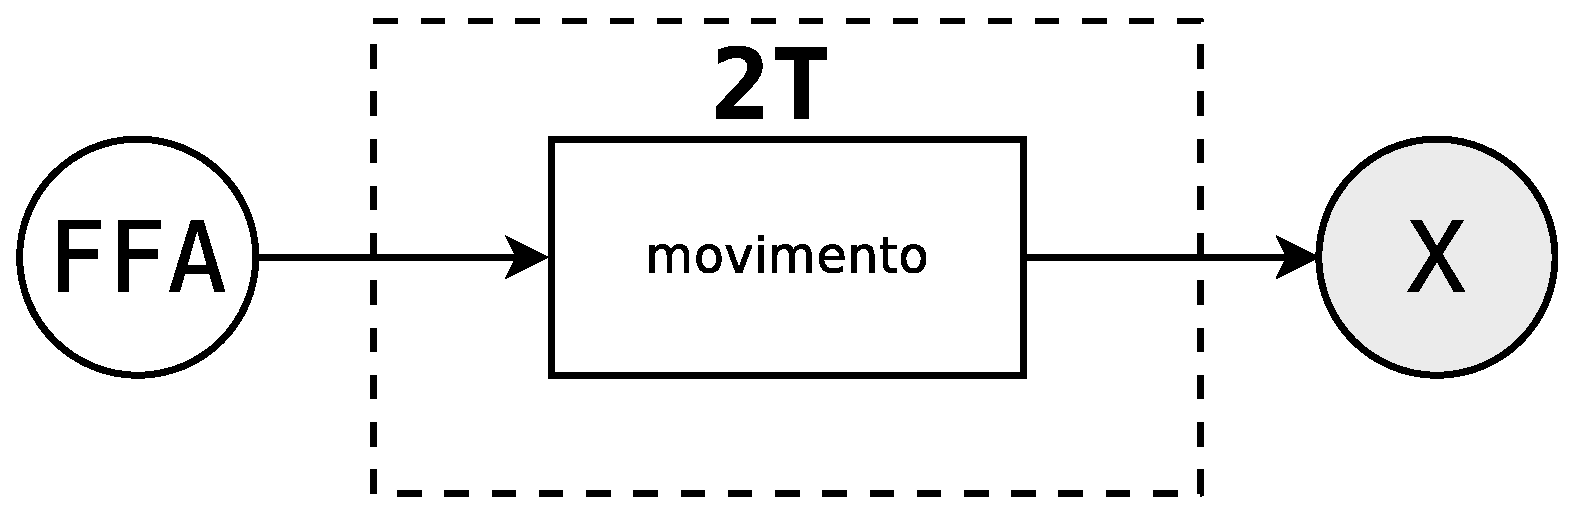
\includegraphics[width=0.5\textwidth]{caps/cap1/saida-lateral.eps}
\caption{Saida lateral (2T).}
\label{fig:passo:saida-lateral}
\end{figure}

\begin{figure}[!h]
\centering 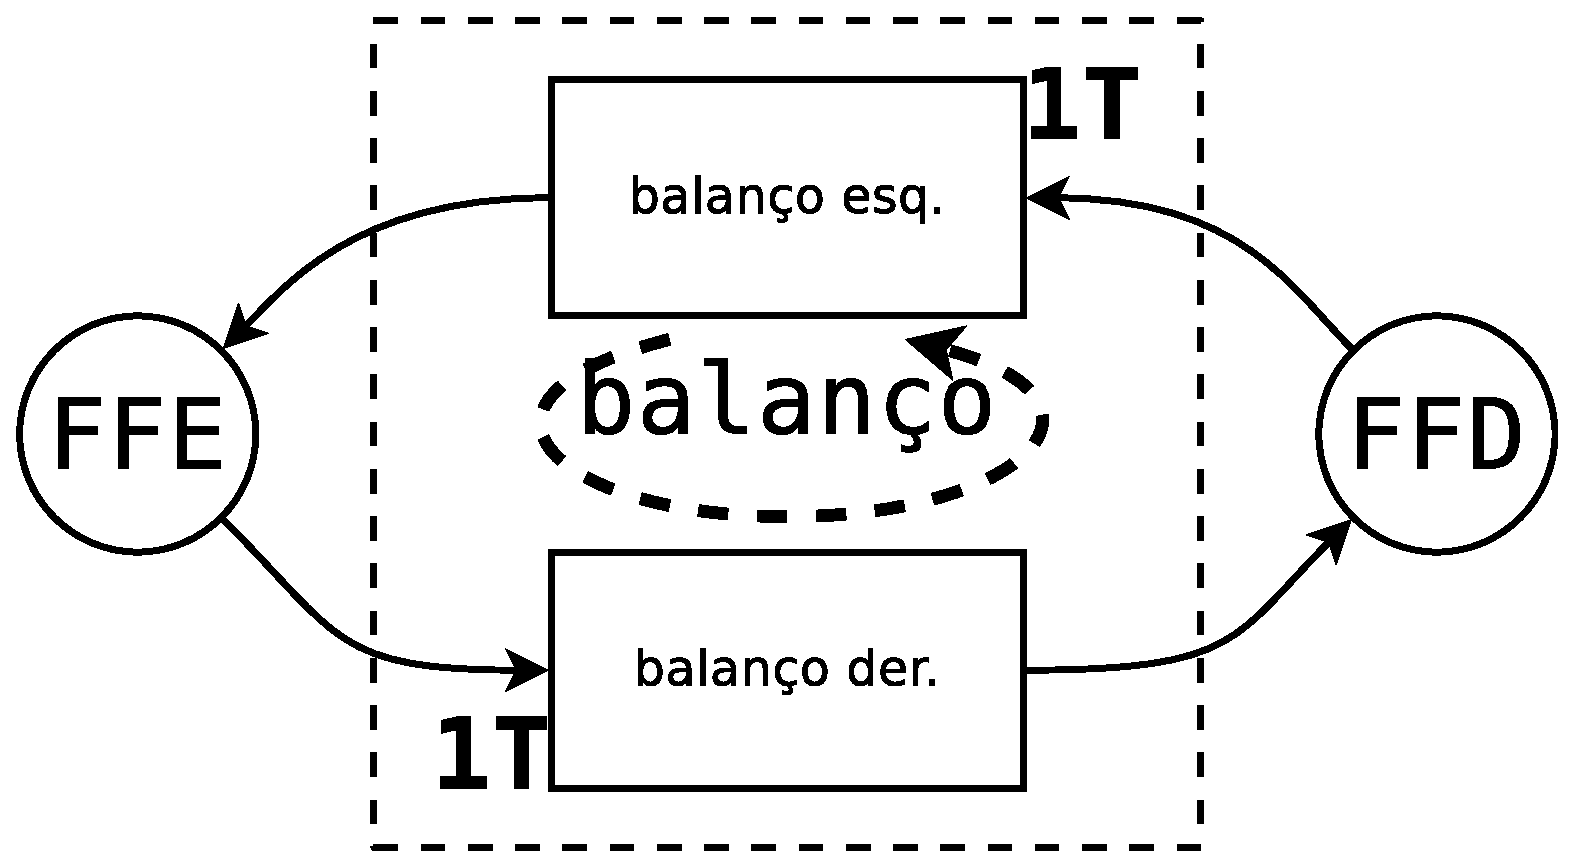
\includegraphics[width=0.5\textwidth]{caps/cap1/balanco.eps}
\caption{Balan�o (2T).}
\label{fig:passo:balanco}
\end{figure}

\begin{figure}[!h]
\centering 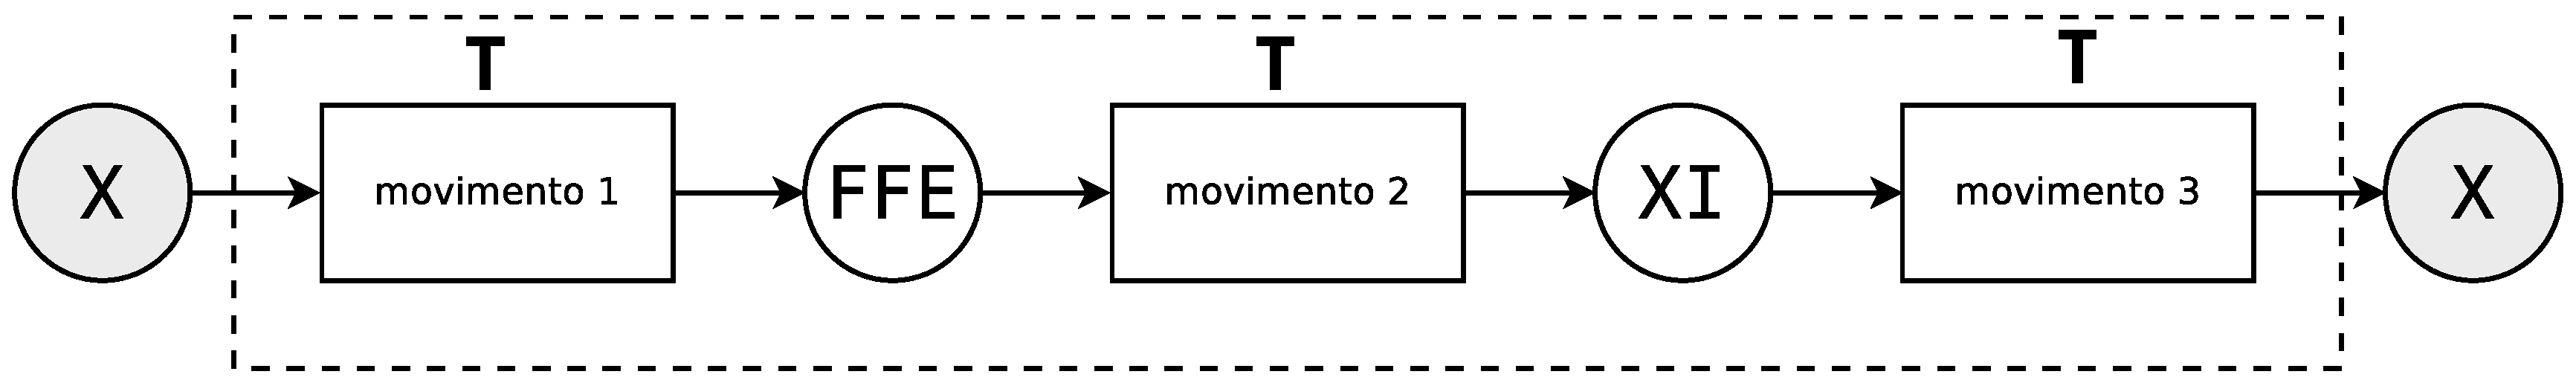
\includegraphics[width=0.99\textwidth]{caps/cap1/caminhada.eps}
\caption{Caminhada (3T).}
\label{fig:passo:caminhada}
\end{figure}

\begin{figure}[!h]
\centering 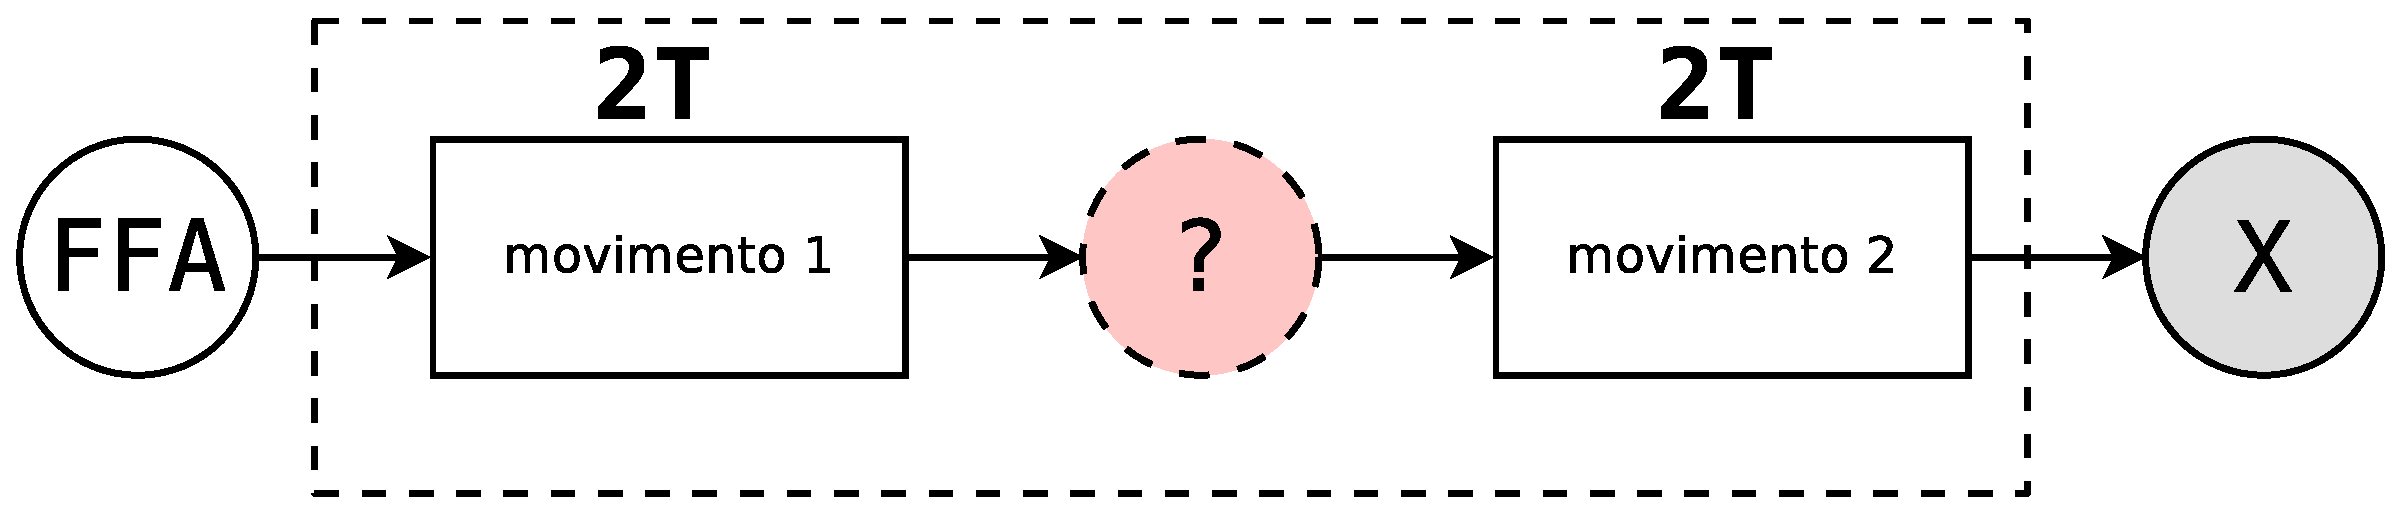
\includegraphics[width=0.7\textwidth]{caps/cap1/giro-da-dama.eps}
\caption{Giro da dama (4T).}
\label{fig:passo:giro-da-dama}
\end{figure}

\begin{figure}[!h]
\centering 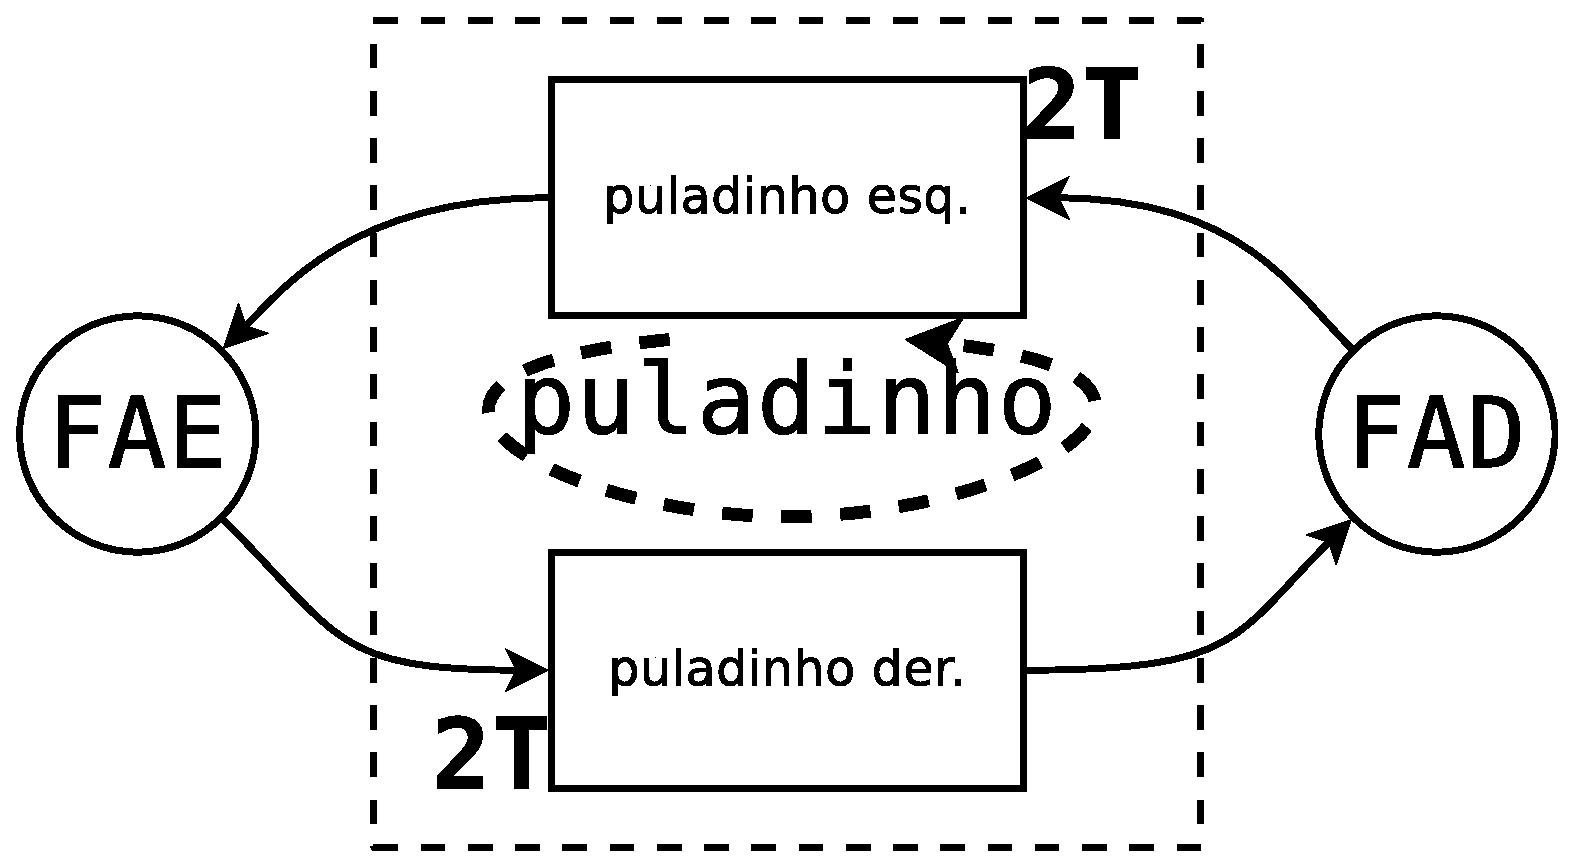
\includegraphics[width=0.5\textwidth]{caps/cap1/puladinho.eps}
\caption{Puladinho (4T).}
\label{fig:passo:puladinho}
\end{figure}

\begin{figure}[!h]
\centering 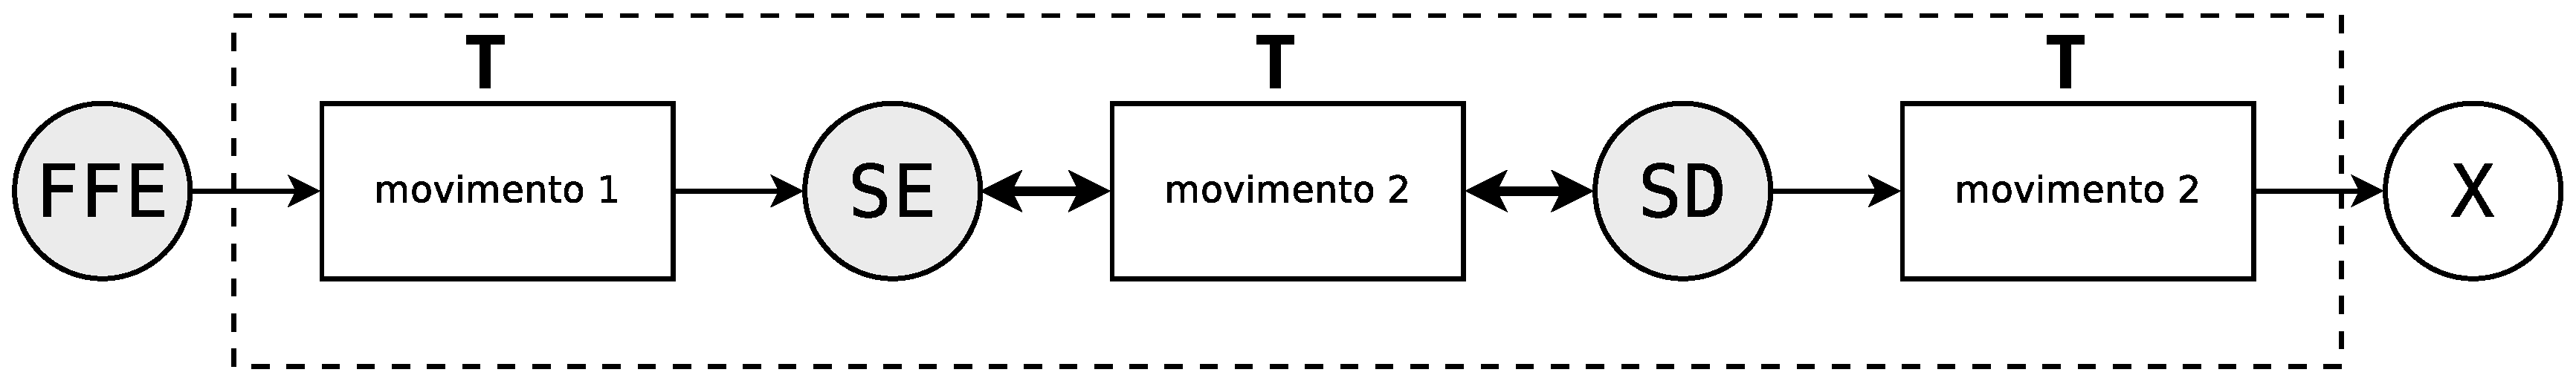
\includegraphics[width=1.0\textwidth]{caps/cap1/esse.eps}
\caption{Esse (3T,5T,...).}
\label{fig:passo:esse}
\end{figure}

\subsection{Passos intermediarios}
\label{sec:passos:intermediarios}

\begin{tasks}(2)
\task Tirada de perna:
\task Rom�rio: Figuras \ref{fig:passo:romario}
\task Gancho redondo:
\task Fac�o:
\task Tran�a (floreado):
\task Assalto (bailarina):
\task Tesoura:
\task Bal�o apagado:
\task Mestre sala
\task Escovinha:
\end{tasks}

\begin{figure}[!h]
\centering 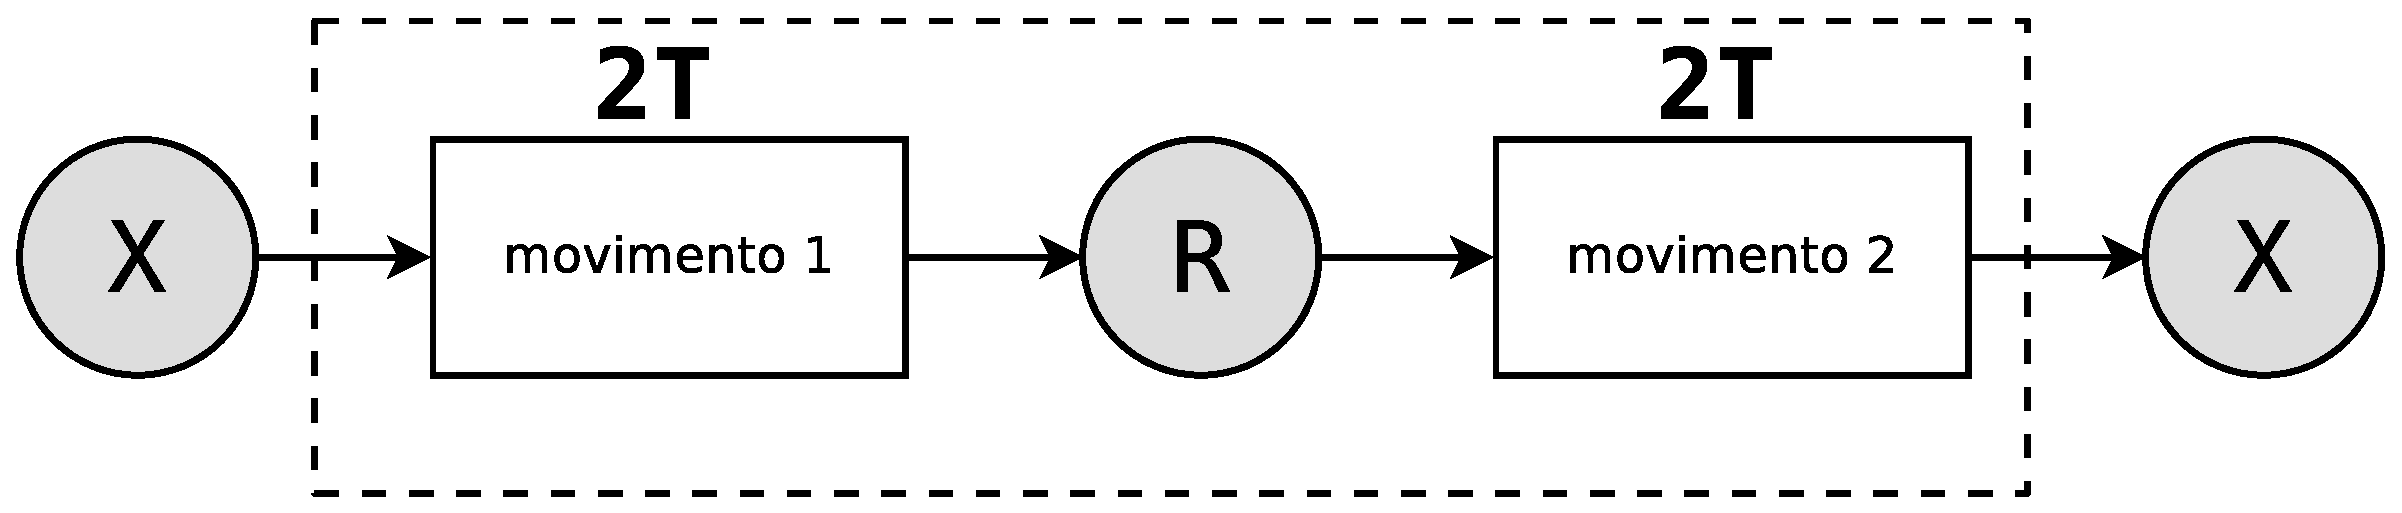
\includegraphics[width=0.7\textwidth]{caps/cap1/romario.eps}
\caption{Romario (4T).}
\label{fig:passo:romario}
\end{figure}

\subsection{Passos avanzados}
\label{sec:passos:avanzados}


\begin{tasks}(2)
\task Pi�o:
\task Picadinho:
\task Bicicleta:
\task Pica-pau:
\task Enceradeira:
\end{tasks}




%% Refer�ncias bibliog�ficas (geradas automaticamente)
\addcontentsline{toc}{chapter}{Referencias bibliogr�ficas}
%\bibliographystyle{plainnat}  %% nome-ano
\bibliographystyle{unsrt}    %% numero
\bibliography{bibliography/bib1}

\appendix
%%Ap�ndice A 
%\include{caps/apendiceA/apA}

\end{document}

